\subsection{Cartes et images}

\begin{figure}[h!]
	\centering
	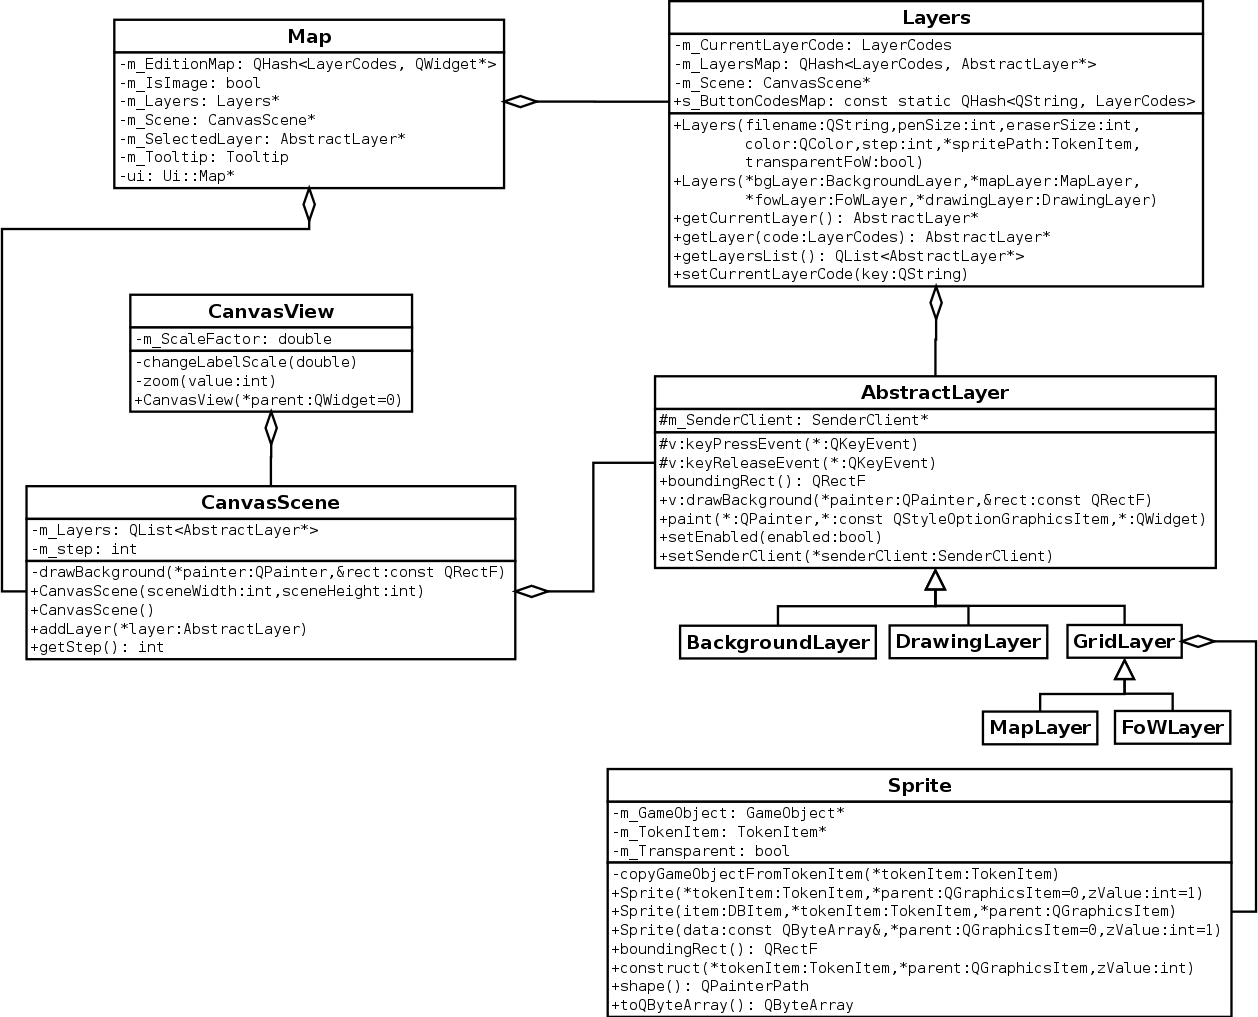
\includegraphics[width=\textwidth]{img/map_uml.png}
	\caption{Diagramme UML de la carte (certaines méthodes sont cachées pour plus de lisibilité)}
\end{figure}

Une image est une carte dont les layers de brouillard de guerre et de personnages sont dissimulés, ainsi que les menus qui leurs sont associés.\\
Une Map hérite de QWidget, afin d'être mise dans une fenêtre, ainsi que de DBItem et SenderHandler pour la mise en réseau. Elle comporte une QGraphicsView, qui sert à afficher une QGraphicsScene comportant différents Layers. Les Layers sont des couches empilées et indépendantes les unes des autres.\\
La classe Map se contente de créer la carte et d'interagir avec la base de données. La création des différents Layers est laissée à la classe Layers, qui possède une QHash associant les layers aux éléments de l'interface utilisateur.\\

Afin d'être placés sur une QGraphicsscene, les Layers sont des QGraphicsObject. Ils sont organisés comme suit:
\begin{description}
	\item[AbstractLayer]: classe abstraite utilisée pour empiler des éléments dans une scène. Réimplémente boundingRect() et paint() de QGraphicsObject. Afin de pouvoir empêcher un Layer d'intercepter les événements, il possède une méthode setEnable(bool) qui permet de déterminer si le boundingRect doit renvoyer la totalité de la scène ou un point nul.
	\item[GridLayer]: classe abstraite utilisée pour positionner des sprites sur la scène, qui seront alignés sur une grille. Gère aussi l'ajout desdits sprites à la BDD. Enfin, elle interprète les évènements de la souris, pour ajouter ou retirer des sprites.
	\item[BackgroundLayer]: hérite directement d'AbstractLayer, et se contente de peindre un arrière plan sur la scène.
	\item[MapLayer]: hérite de GridLayer, et sert à positionner les jetons sur la carte. En plus de réimplémenter la gestion des événements à la souris, ce Layer gère des actions de drag and drop. Il  permet aussi d'afficher les informations sur les sprites (points de vie et hauteur de la pile de jetons).
	\item[FoWLayer]: hérite de GridLayer, et sert à positionner les sprites de brouillard de guerre. Ces sprites peuvent être opaques ou transparents selon la valeur d'un booléen dans le constructeur. Ce Layer ne modifie pas l'interprétation des événements de la souris de GridLayer. Possède deux méthodes pour remplir ou vider la carte de son brouillard de guerre. 
	\item[DrawingLayer]: hérite directement de AbstractLayer. Contient une QPixmap, originellement vide, sur laquelle l'utilisateur pourra dessiner. Afin de gérer les événements de la souris de manières complètement différentes, ce Layer installe les eventFilter depuis des Tools. Ces Tools sont organisés de manière similaires aux Layers: une classe AbstractTool, différentes classes concrètes de Tools, et une liste Tools qui construit les Tools et permet de les associer à un bouton de l'interface graphique.
\end{description}